L'étape de compilation doit permettre de transcrire la liste linéarisée de \pyinline{StructureNode} obtenue à l'issue de la phase d'analyse (\cref{sec:ParsedCode}) dans le code assembleur et le code binaire correspondant au modèle de processeur retenu (\cref{sec:processeur}).

\subsubsection{Classe CompilationManager}

La compilation est assurée par une instance de la classe \pyinline{CompilationManager}. Le code assembleur, le binaire et les méthodes associées sont gérés par une instance de la classe \pyinline{AssembleurContainer}.

Pour chaque \pyinline{StructureNode}, \pyinline{CompilationManager.__pushNodeAsm} détermine le type de n\oe ud et délègue à l'instance \pyinline{AssembleurContainer} la création du code assembleur et binaire correspondant.

Lorsque le n\oe ud nécessite l'évaluation d'une expression arithmétique ou d'une comparaison, la compilation est gérée par une instance de la classe \pyinline{CompileExpressionManager}

\begin{figure}[h!]
	\vspace{-1cm}
	\centering
	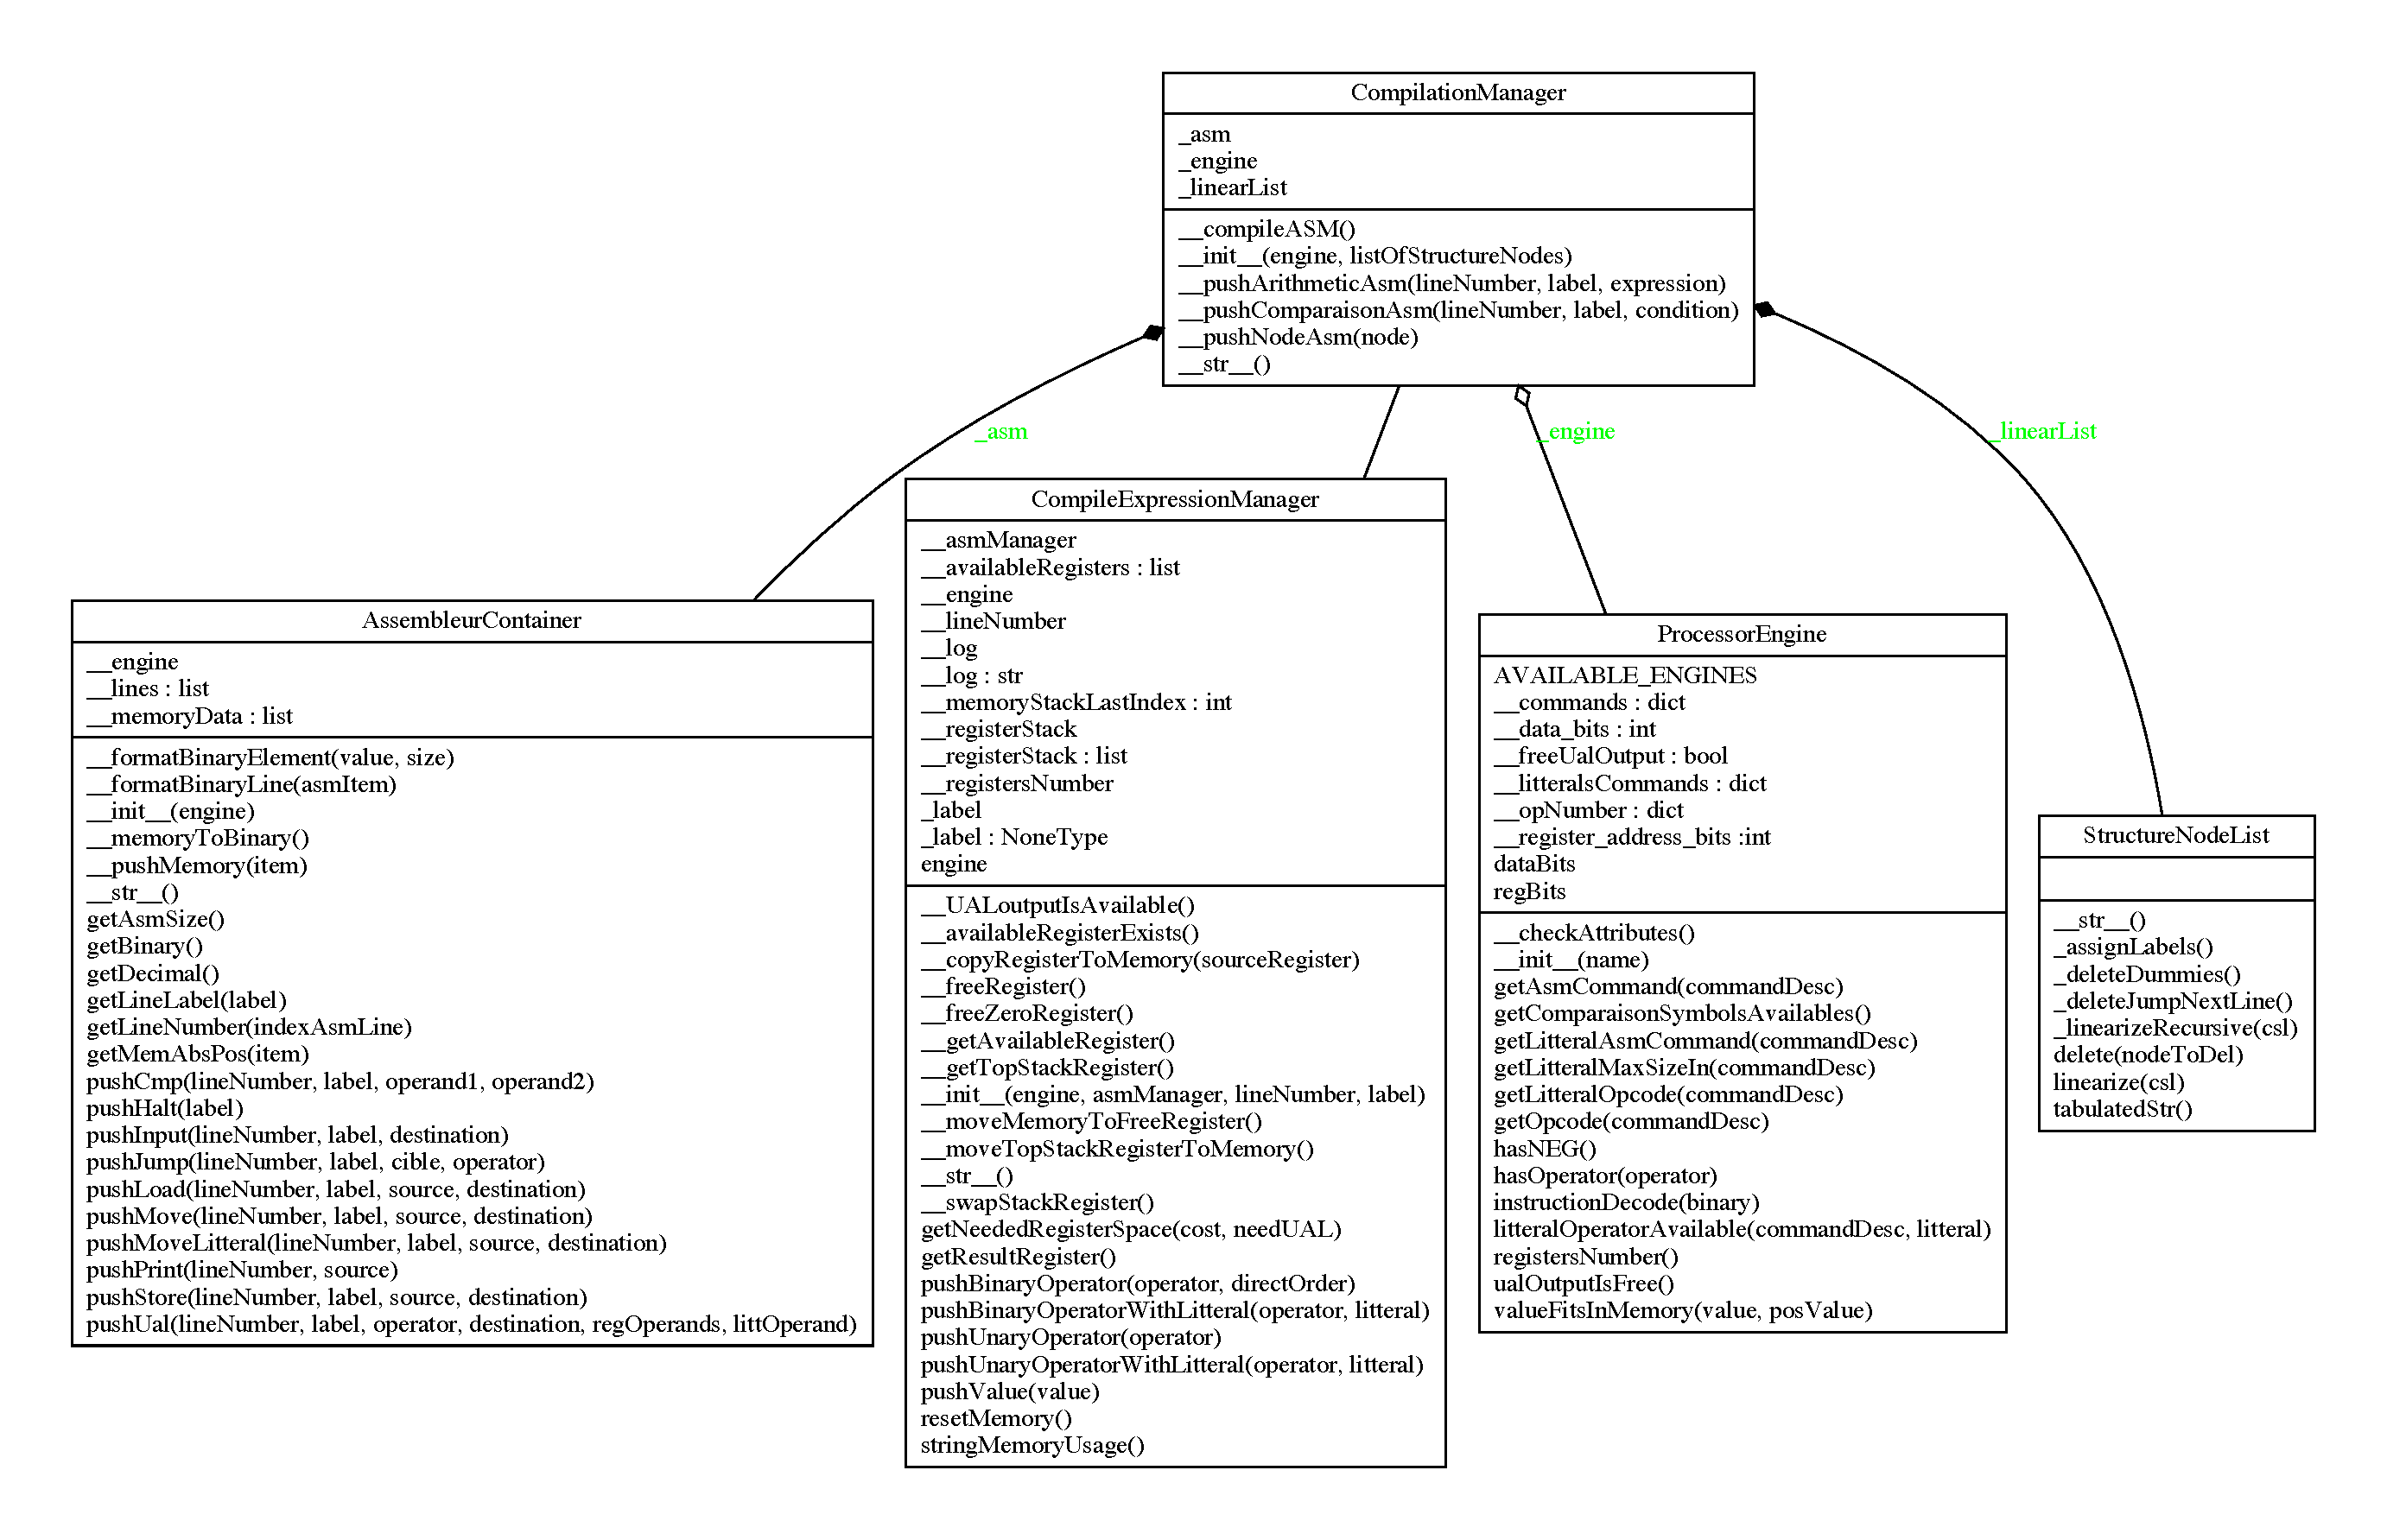
\includegraphics[width=\textwidth]{./Pictures/CompilationManager.pdf}
	\caption{\label{fig:class_CompileManager}Diagramme de classes - Compilation}
\end{figure}

\subsubsection{CompileExpressionManager}
\pyinline{CompilationManager} délègue à la classe\pyinline{CompileExpressionManager} la production du code assembleur liée aux expressions arithmétiques et aux comparaisons. En particulier tout ce qui concerne:
\begin{itemize}
	\item la gestion des registres et pile de registre,
	\item la gestion de mémoire et pile mémoire,
	\item les transferts entre registres et mémoire.
\end{itemize}


\subsubsection{AssembleurContainer}
\pyinline{AssembleurContainer} a en charge l'ensemble des opérations liées à la manipulation aux codes assembleur et binaire (transtypage, conversion) ainsi que la responsabilité de la production du code pour les objets de type \pyinline{StructureNode}.
